\section{The numerator tables}\label{app:tables}

\begin{proposition}\label{prop:num}
For $p=\alpha/(\alpha+\beta)$ and $N\ge1$, the numerators of Remark~\ref{rem:tables} are
$n_N(k)=\sum_{w}\alpha^{\rep(w)}\beta^{\chg(w)}$, summed over the words with $k$ letters $\sR$ and
$N-k$ letters $\sL$. So they are integers, and
\[
\sum_{a,b\ge0}n_{a+b}(a)\,x^ay^b=
\frac{1-(\alpha-1)(x+y)+(\alpha-\beta)(\alpha+\beta-2)\,xy}{1-\alpha(x+y)+(\alpha^2-\beta^2)\,xy}.
\]
\end{proposition}

\begin{proof}
Multiply \eqref{eq:wordprob} by $2(\alpha+\beta)^{N-1}$. Let $H_{\sR}$ and $H_{\sL}$ be the weighted
sums over the words ending in $\sR$ and in $\sL$, with $x$ marking $\sR$ and $y$ marking $\sL$. Then
$H_{\sR}=x(1+\alpha H_{\sR}+\beta H_{\sL})$ and $H_{\sL}=y(1+\alpha H_{\sL}+\beta H_{\sR})$, and solving as in
the proof of Proposition~\ref{prop:gf} gives $1+H_{\sR}+H_{\sL}$.
\end{proof}

For $(\alpha,\beta)=(2,1)$ this is $(1-x)(1-y)/(1-2x-2y+3xy)$, and for $(1,2)$ it is
$(1-xy)/(1-x-y-3xy)$, the generating functions recorded in A035002 and
A348595~\cite{oeisA035002,oeisA348595}. Figure~\ref{fig:lattice} shows both bijections.

\begin{figure}[ht]
\centering
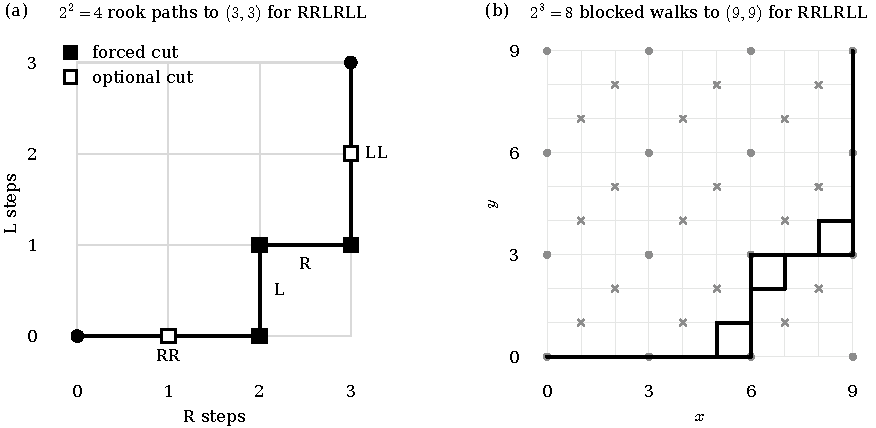
\includegraphics{figures/lattice}
\caption{The 2 bijections for the word $\sR\sR\sL\sR\sL\sL$. (a) The rook path. A cut
is forced at each of the $3$ direction changes (filled) and optional between
equal letters (hollow), so the word comes from $2^2=4$ rook paths to $(3,3)$.
(b) The union of the $2^3=8$ blocked walks to $(9,9)$ that give the word,
with 1 detour square for each direction change. Blocked points are marked
$\times$ and corners by dots.}
\label{fig:lattice}
\end{figure}

\begin{theorem}[$p=\tfrac23$ and rook paths]\label{thm:rook}
Let $r(a,b)$ count the rook paths from $(0,0)$ to $(a,b)$ with every move to the right or up. For
$p=\tfrac23$, $n_N(k)=r(k,N-k)$ for all $0\le k\le N$. Since the array of A035002 starts at $(1,1)$,
Kagey's $p=\tfrac23$ table read by rows is A035002 read by antidiagonals.
\end{theorem}

\begin{proof}
By definition each entry of A035002 is the sum of the entries to its left and above it, which is the
recursion for $r$ obtained by removing the last move. A rook path to $(a,b)$ with $a+b=N\ge1$ gives
a word $w$ with $a$ letters $\sR$ and $b$ letters $\sL$, one letter per unit of length, and a set of
cuts $i<N$ where one move ends and the next begins. A cut is forced where $w_i\ne w_{i+1}$ and
optional where $w_i=w_{i+1}$, and each choice of optional cuts gives exactly one rook path. Hence,
$r(a,b)=\sum_w2^{\rep(w)}$, which is $n_N(a)$ for $(\alpha,\beta)=(2,1)$ by
Proposition~\ref{prop:num}.
\end{proof}

\begin{theorem}[$p=\tfrac13$ and Mathar's blocked walks]\label{thm:mathar}
Call $(x,y)$ \emph{blocked} if $x\equiv y\equiv1$ or $x\equiv y\equiv2\pmod 3$, and let $M(a,b)$
count the walks from $(0,0)$ to $(3a,3b)$ with unit steps right and up that avoid blocked points.
For $p=\tfrac13$, $n_N(k)=M(k,N-k)$. The array $M$ is symmetric.
\end{theorem}

\begin{proof}
Work modulo $3$ and call a point with residue $(0,0)$ a \emph{corner}. Since $(1,1)$ and $(2,2)$ are
blocked, a right step from a corner is followed by another, to $(2,0)$, which we call state
$\mathsf A$, and an up step leads on to $(0,2)$, state $\mathsf B$. From $\mathsf A$ the walk steps
right to a corner, or it goes up, right and up to $\mathsf B$, and $\mathsf B$ behaves symmetrically. Leaving
$\mathsf A$ crosses one line $x\equiv0$ and no line $y\equiv0$, leaving $\mathsf B$ does the
reverse, and leaving a corner crosses neither. A walk to $(3a,3b)$ crosses $a$ lines $x\equiv0$ and
$b$ lines $y\equiv0$, so writing $\sR$ for each visit to $\mathsf A$ and $\sL$ for each visit
to $\mathsf B$ gives a word $w$ with $a$ letters $\sR$ and $b$ letters $\sL$. Between $w_i$ and $w_{i+1}$
the walk passes through a corner if $w_i=w_{i+1}$, in 1 way, and through a corner or directly if
$w_i\ne w_{i+1}$, in 2 ways. The start and the end are forced. Hence $M(a,b)=\sum_w2^{\chg(w)}$,
which is $n_N(a)$ for $(\alpha,\beta)=(1,2)$ by Proposition~\ref{prop:num}. Swapping the letters
$\sR$ and $\sL$ keeps $\chg(w)$, so $M(a,b)=M(b,a)$.
\end{proof}

In Mathar's note~\cite{mathar2022} the ``squares'' of A348595 are lattice points. A direct count
of the walks gives its published terms (computer-checked, Section~\ref{sec:verify}). So A348595
lists the lower triangle of $M$, which is how that entry is ``related'' to the $p=\tfrac13$ table.
